\section{DGF-Bench: measured review performance on 300 synthetic projects}
\label{sec:benchmark}

\subsection{Question, population, and information available to the agents}

This experiment asks whether an AI agent can apply a declared governance policy, identify the
required findings and actions, cite observed evidence, respect its authority, and carry a review
through a connected route. It measures review decisions and proposed actions, not implementation
of remediation or changes in human workload. It is distinct from the prospective enterprise and
factorial studies in Section~\ref{sec:testing}.

The dataset contains 300 fictional projects: 100 Buy, 100 Integrate, and 100 Build cases.
Buy and Integrate contain six gate occurrences each, and Build contains five, for 1,700 occurrences
per model and 5,100 planned observations across three models. Cases were generated before these
evaluations at difficulty setting 4, with sampling conditioned to improve decision coverage.
Project context, owners, budgets, data classifications, technical architectures, documents, and
simulated system records derive from canonical case facts. Documents can be missing, stale, or
inconsistent. Specialist reviews precede a final General review; the routes are examples rather
than a universal enterprise standard.

The agent receives gate objectives, a structured output contract, an explicit decision policy,
and tools to read allowed evidence and query the synthetic environment. In particular, the policy
includes executable rule definitions and identifies an authoritative structured
\texttt{REVIEW\_FACTS} snapshot. The evaluator-only reference file is inaccessible through the
agent's tools. This is nevertheless a strongly scaffolded test of policy application: the agent
need not discover the rules or reconstruct every decision-relevant fact from unstructured documents.
Architecture images are available under the vision setting; image availability is not evidence
that image interpretation was necessary for success. These design choices limit claims about
expert reasoning on independently collected enterprise dossiers.

The dataset audit reports 300 distinct project identifiers, architecture signatures, and complete
decision-fact signatures, but only 267 distinct whole-case finding patterns. Gate-specific relevant
fact signatures include 142 of 200 Compliance cases and 241 of 300 Security cases. All rules
applicable to the selected phases are covered according to the generator's audit. Phase-adjusted
normalized decision entropy ranges from 0.9971 to 1.0000. Balanced labels improve coverage, but
do not estimate enterprise prevalence or establish independent business validity.

\subsection{Protocol, completion, and outcomes}

The requested OpenRouter identifiers were \nolinkurl{deepseek/deepseek-v4.1-flash},
\nolinkurl{google/gemini-3.8-flash}, and \nolinkurl{openai/gpt-5.6-luna}. Configuration was temperature
0, vision \texttt{auto}, agent-produced handoffs, at most 20 turns and 40 tool calls per gate,
and 8,192 output tokens per turn. Gates remained sequential within a project. The last resume
used 12 workers, four per model, and a USD~110 cost cap; an earlier invocation used six workers
and a USD~65 cap. Data collection spanned 22--23 September 2026. Resumption retained completed
cases and valid gate checkpoints. Historical provider/key-limit failures remain in the released
traces. The 78.73-minute elapsed time in the last run statistics describes that resume only.

Of 900 planned model--case runs, 899 are evaluable: 300 for DeepSeek, 299 for Gemini, and 300
for Luna. Gemini case \nolinkurl{DGF-INT-035128_integrate} failed at its first IT gate with
a provider generation error (\texttt{finish\_reason=error}); it is excluded as an infrastructure failure. Thus 5,094 of 5,100
planned gates are evaluable, with all expected gates attempted in the evaluable cases. There
are no recorded final agent-protocol failures or model-identifier mismatches. Provider-reported
identity is not an independent audit of underlying weights. DeepSeek was served by multiple
OpenRouter providers; Gemini and Luna were recorded through Google AI Studio and OpenAI.

Scoring uses \texttt{DGF-decision-v8.2-authorized-review}. A gate succeeds strictly only if its
disposition, finding set, action set, evidence provenance, and authorization indicator all satisfy
the reference. Findings and actions require F1 equal to one. Evidence requires an observed
reference and exact excerpts supporting the relevant field/value tokens. This is lexical
provenance checking, not independent verification of arbitrary reasoning. Authorized conditional
approvals can change the effective reference disposition; the evaluator verifies the mandate
and recorded action. General combines effective reference opinions, so an upstream error can
also cause a downstream failure. Complete-route success requires every gate to succeed strictly;
it does not mean that remediation was executed.

Gate confidence intervals use a route-stratified bootstrap of whole cases, preserving dependence
between a project's gates (2,000 draws, seed 81931; a case-count Wilson fallback handles degenerate
intervals). Route intervals use Wilson bounds. Pairwise differences use the same 299 cases for
all models, resampled together within routes (10,000 draws, NumPy seed 81931). These are descriptive
intervals conditional on the synthetic sampling design. No preregistered analysis or independently
adjudicated ground truth is claimed, and one trajectory per model and case does not estimate
run-to-run inference variability.

\subsection{Overall and route-level results}

\begin{table}[!htb]
\centering\small
\caption{Measured synthetic benchmark outcomes. Gate CSR requires complete conformity; route success requires all gates. Cost includes recorded failed attempts.}
\label{tab:bench-overall}
\begin{tabularx}{\linewidth}{@{}l r L L r@{}}
\toprule
Model & Cases & Gate CSR [95\% CI] & Route success [95\% CI] & USD\\
\midrule
\rowsinput{generated/table_benchmark_overall}
\bottomrule
\end{tabularx}
\end{table}

Gemini succeeds strictly on 1,609 of 1,694 gates, Luna on 1,416 of 1,700, and DeepSeek on
1,261 of 1,700. Corresponding complete-route counts are 230 of 299, 127 of 300, and 74 of 300
(Table~\ref{tab:bench-overall}). Mean weighted component scores, which are not strict success
rates, are 99.68\%, 97.67\%, and 95.02\%, respectively. The distinction matters: strong average
components can coexist with many incomplete project reviews.

\begin{figure}[!htb]
\centering
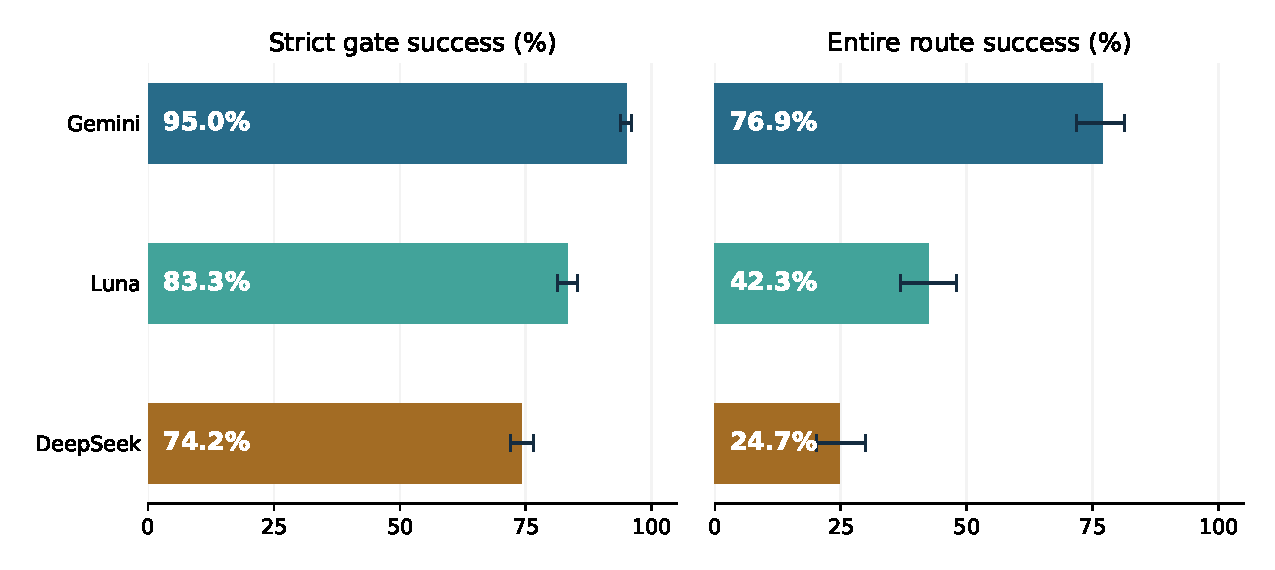
\includegraphics[width=\linewidth]{figures/fig_benchmark_results.pdf}
\caption{Measured review outcomes and recorded cost. Intervals are computed over independent
case units rather than treating all gates as independent trials. These are model observations
on synthetic dossiers, separate from the workforce scenario figures.}
\label{fig:benchmark-results}
\end{figure}

On the 299 common cases, CSR is 94.98\% for Gemini, 83.23\% for Luna, and 74.09\% for DeepSeek.
Paired differences are 20.90 percentage points for Gemini minus DeepSeek (95\% interval
18.30--23.44), 11.75 for Gemini minus Luna (9.62--13.93), and 9.15 for Luna minus DeepSeek
(6.67--11.63). The ranking persists on the matched cohort; this is not a universal model ranking.

\begin{table}[!htb]
\centering\small
\caption{CSR and complete-route counts by project route. Gemini excludes one Integrate case.}
\label{tab:bench-routes}
\begin{tabularx}{\linewidth}{@{}l L L L@{}}
\toprule
Route & DeepSeek: CSR; routes & Gemini: CSR; routes & Luna: CSR; routes\\
\midrule
\rowsinput{generated/table_benchmark_routes}
\bottomrule
\end{tabularx}
\end{table}

Gemini's route success falls from 87 of 100 Buy cases to 68 of 100 Build cases. Luna succeeds
on 20 Buy, 52 Integrate, and 55 Build cases; DeepSeek succeeds on 13, 32, and 29, respectively
(Table~\ref{tab:bench-routes}). These differences do not isolate the causal effect of route
length, because gate composition and case content also differ.

\begin{table}[!htb]
\centering\small
\caption{Strict success by gate family (percent). Counts vary by route composition; complete
denominators and intervals are supplied in the released tables.}
\label{tab:bench-gates}
\begin{tabular}{@{}l r r r@{}}
\toprule
Gate & DeepSeek & Gemini & Luna\\
\midrule
\rowsinput{generated/table_benchmark_gates}
\bottomrule
\end{tabular}
\end{table}

Procurement is the lowest-CSR gate for both Luna (33\%) and DeepSeek (43\%). Luna's General
CSR is 61.67\%. Luna exceeds Gemini's descriptive CSR in Architecture and Tech Readiness
(Table~\ref{tab:bench-gates}); these local comparisons are exploratory, without multiplicity-adjusted
tests or a claim of specialist superiority.

\subsection{Evidence failures, unsafe approvals, and cost}

Disposition accuracy alone is 100\% for Gemini, 98.12\% for Luna, and 95.24\% for DeepSeek.
All 85 Gemini strict failures concern evidence conformity; findings, actions, dispositions, and
authorization indicators match the reference. Evidence is the sole failing component in 221 of
284 Luna failures and 338 of 439 DeepSeek failures. Invalid excerpts and missing or unobserved
references are grouped by these diagnostics; not all are harmless formatting defects. Changing
the evidence rule after observing results would change the estimand. A semantic evidence metric
would require a separately declared analysis.

DeepSeek records one critical finding miss and one false approval, both in the Architecture
review of \texttt{DGF-INT-035136\_integrate}. An address overlap required \texttt{NO\_GO}; at
forced finalization, the model submitted \texttt{GO} with an empty finding set, no evidence, and
a ``placeholder'' rationale. The response passed the submission schema but failed the substantive
score. This observation combines decision quality with the ability to finalize under resource limits.

Luna records three critical misses and one false approval. In case
\texttt{DGF-INT-035197\_integrate}, its Legal review approved a dossier with a missing DPA,
while its own rationale said that \texttt{REWORK} was required. The other critical misses concern
private endpoints in Security and an upstream \texttt{NO\_GO} in General. The latter can include
error propagation and should not be interpreted as an independent new safety event. Gemini has
no observed critical miss or false approval in its evaluable runs; this does not establish zero
risk. Recorded truncated-response counts are 2 for DeepSeek, 14 for Gemini, and 0 for Luna,
without implying that these counts equal incomplete cases.

The usage ledgers sum to USD~87.015829172, agreeing with the cumulative budget counter.
Gemini accounts for USD~71.88, DeepSeek USD~10.09, and Luna USD~5.05, including recorded retries
and failures. Approximate cost per evaluated dossier is USD~0.240, 0.034, and 0.017, respectively.
Luna therefore combines a higher overall strict score with lower recorded cost than DeepSeek
in this execution. Costs depend on provider routing, caching, price, and retry history; they are
not a labor-cost comparison or a permanent pricing claim.

\subsection{Interpretation and reproducibility boundary}

The experiment demonstrates high disposition agreement with an explicit rule system, alongside
material losses when complete evidence-bearing routes are required. It supplies no direct
estimate of review hours saved, autonomous remediation, production acceptance, human equivalence,
or the 2033 FTE hypothesis. The generator and evaluator share rules, facts are deliberately
structured, decisions are balanced, and there is no human baseline or independent expert
adjudication. Policy-application results should not be generalized to tacit rules, adversarial
inputs, private enterprise populations, or complete governance automation.

The published release preserves all files of the recorded run and its dataset, including old
failed attempts, the original partial exports, and the final analysis. Only the final analysis
tables describe the 899 evaluable runs. Frozen benchmark sources reproduce the recorded source
fingerprint; the repository's evolving default branch is not substituted for them. Five targeted
offline rescoring checks reproduced the saved gate scores exactly, including all cases with critical
misses, and all 899 score files passed internal count consistency checks. These checks establish
reproducibility of this evaluator, not independent validation of its governance judgments.
